\section{experiments}

	4 big experiments have been executed.
	
	\begin{itemize}
		\item noise analysis
		\item tracking, manually changing the set points
		\item tracking using sine/stair functions
		\item disturbances
	\end{itemize}

\subsection{simulink}
	\begin{figure}[H]
	\centering
	\begin{subfigure}[b]{0.45\textwidth}
		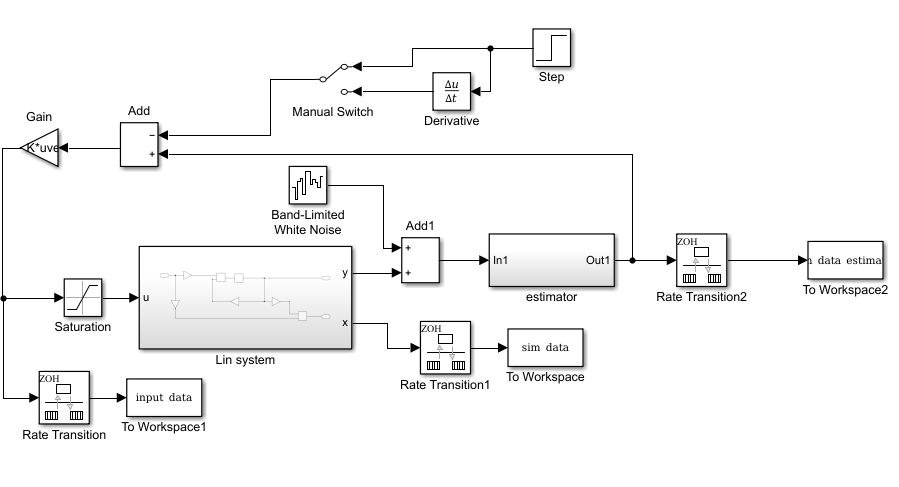
\includegraphics[width=\textwidth]{./part4_experiments/not_generated/simulink_main.png}
		\caption{main diagram}
	\end{subfigure}
	\begin{subfigure}[b]{0.45\textwidth}
		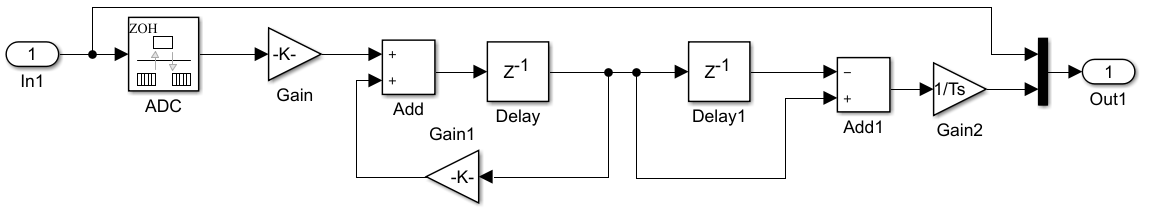
\includegraphics[width=\textwidth]{./part4_experiments/not_generated/simulink_estimator.png}
		\caption{estimator}
	\end{subfigure}
	\caption{simulink diagram}
\end{figure}
\subsection{noise analysis}
	$\theta$ and $\alpha$ have been measured before and after the low pass filter. The difference between those signals is considered noise as displayed in figure~\ref{fig:time plot noise}. Instead of looking at the noise in function of time its very useful to look at a histogram as is done in figure~\ref{fig:hist noise}. The variance of the noise can easily be calculated and then used in the simulation.
	
	\begin{figure}[H]
		\centering
		\begin{subfigure}[b]{0.45\textwidth}
			\includegraphics[width=\textwidth]{./part4_experiments/noise/simple_plot.png}
			\caption{time plot of $\theta$ and $\alpha$ before and after the low pass filter}
			\label{fig:time plot theta and alpha}
		\end{subfigure}
		\begin{subfigure}[b]{0.45\textwidth}
			\includegraphics[width=\textwidth]{./part4_experiments/noise/difference.png}
			\caption{Difference of $\theta$/$\alpha$ before and after the low pass filter}
			\label{fig:time plot noise}
		\end{subfigure}
		\begin{subfigure}[b]{0.45\textwidth}
			\includegraphics[width=\textwidth]{./part4_experiments/noise/histogram.png}
			\caption{Historgram of the noise}
			\label{fig:hist noise}
		\end{subfigure}
	\end{figure}

\subsection{manual tracking}
	\begin{figure}[H]
		\centering
		\begin{subfigure}[b]{0.45\textwidth}
			\includegraphics[width=\textwidth]{./part4_experiments/tracking_manual/alpha_theta.png}
			\caption{states $\theta$ and $\alpha$}
		\end{subfigure}
		\begin{subfigure}[b]{0.45\textwidth}
			\includegraphics[width=\textwidth]{./part4_experiments/tracking_manual/alpha_theta_dot.png}
			\caption{states $\dot{\theta}$ and $\dot{\alpha}$}
		\end{subfigure}
		\begin{subfigure}[b]{0.45\textwidth}
			\includegraphics[width=\textwidth]{./part4_experiments/tracking_manual/motor_input.png}
			\caption{motor input}
		\end{subfigure}
	\end{figure}
\subsection{tracking}
	\begin{figure}[H]
		\centering
		\begin{subfigure}[b]{0.45\textwidth}
			\includegraphics[width=\textwidth]{./part4_experiments/tracking_sine/alpha_theta.png}
			\caption{states $\theta$ and $\alpha$}
		\end{subfigure}
		\begin{subfigure}[b]{0.45\textwidth}
			\includegraphics[width=\textwidth]{./part4_experiments/tracking_sine/alpha_theta_dot.png}
			\caption{states $\dot{\theta}$ and $\dot{\alpha}$}
		\end{subfigure}
		\begin{subfigure}[b]{0.45\textwidth}
			\includegraphics[width=\textwidth]{./part4_experiments/tracking_sine/motor_input.png}
			\caption{motor input}
		\end{subfigure}
		\caption{tracking with a sine wave}
	\end{figure}

	\begin{figure}[H]
		\centering
		\begin{subfigure}[b]{0.45\textwidth}
			\includegraphics[width=\textwidth]{./part4_experiments/tracking_stair/alpha_theta.png}
			\caption{states $\theta$ and $\alpha$}
		\end{subfigure}
		\begin{subfigure}[b]{0.45\textwidth}
			\includegraphics[width=\textwidth]{./part4_experiments/tracking_stair/alpha_theta_dot.png}
			\caption{states $\dot{\theta}$ and $\dot{\alpha}$}
		\end{subfigure}
		\begin{subfigure}[b]{0.45\textwidth}
			\includegraphics[width=\textwidth]{./part4_experiments/tracking_stair/motor_input.png}
			\caption{motor input}
		\end{subfigure}
		\caption{tracking with a stair function}
	\end{figure}

\subsection{disturbances}
	\begin{figure}[H]
		\centering
		\begin{subfigure}[b]{0.45\textwidth}
			\includegraphics[width=\textwidth]{./part4_experiments/disturbance_rejection/alpha_theta.png}
			\caption{states $\theta$ and $\alpha$}
		\end{subfigure}
		\begin{subfigure}[b]{0.45\textwidth}
			\includegraphics[width=\textwidth]{./part4_experiments/disturbance_rejection/alpha_theta_dot.png}
			\caption{states $\dot{\theta}$ and $\dot{\alpha}$}
		\end{subfigure}
		\begin{subfigure}[b]{0.45\textwidth}
			\includegraphics[width=\textwidth]{./part4_experiments/disturbance_rejection/motor_input.png}
			\caption{motor input}
		\end{subfigure}
		\caption{disturbance rejection test}
	\end{figure}